\documentclass[a4paper,12pt,twoside]{report}
\usepackage[left=2.7cm,right=2.7cm,top=2cm,bottom=3cm]{geometry}
%\usepackage[square,authoryear,sort]{natbib}
\usepackage{url}
\usepackage{xcolor}
\usepackage{graphicx}
\usepackage{pdfpages}

\makeatletter
\def\@makechapterhead#1{%
  \vspace*{50\p@}%
  {\parindent \z@ \raggedright \normalfont
    \interlinepenalty\@M
    \Huge\bfseries  \thechapter.\quad #1\par\nobreak
    \vskip 40\p@
  }}
\makeatother

\makeatletter
\newcommand*{\toccontents}{\@starttoc{toc}}
\makeatother


\let\endtitlepage\relax
\begin{document}

\title{\LARGE {\bf Anomaly Detection in Computer Networks - Literature Review}\\
 \vspace*{6mm}
}

\author{Henry Clausen}
%\date{October 2008}

\maketitle

\toccontents
%\begin{abstract}
%Text
%\end{abstract}


\chapter{Overview}

\section{Network attacks}

Sophisticated data breaches affect hundreds of million customers and inflicts tremendous financial, reputational, and logistic damage. %Cyber-security incidents increased by 38\% in 2017, and the global cost of cyber crime is estimated to reach \$2 trillion by 2019 %\citep{conteh2016rise}. The prevention of cyber crime is therefore a globally demanded necessity.
One reason for the recent rise of cyber crime is the increased use of sophisticated techniques for the attack of specific targets. Attackers use customised social engineering and custom-build malware that penetrate defensive barriers and potentially stay undetected in an infected system for an extended period of time. 



%Existing solutions to commercial intrusion detection in computer networks are often based on \textbf{detecting signatures} of previously uncovered and analysed  attacks. Examples of such signatures include  file  hashes of malicious software, blacklisted IP addresses and domain names, and characteristics of known Command-and-Control (C\&C) protocols. Detection of a signature usually indicates an imminent intrusion and triggers investigation. 



%However, with attackers becoming adept at shedding such previously identified signatures, cyber-security researchers have to find ways of quantifying malicious activity in a more robust way. 

%However, attackers are becoming more adept at shedding previously gathered signatures: A file hash can be altered by minor modifications in the program and IP and domain addresses can be switched by changing servers. A sophisticated attack will employ new, customized protocols and software that is fitted to the targeted computer infrastructure, and thus will not show any identified signatures. 

%The field of \textit{Intrusion Detection} is concerned with the development of methods and tools that identify malicious behaviour in a computer network in a more robust way. %\textcolor{red}{In this work, I will discuss existing literature concerning a sub-branch intrusion detection, that is concerned with detecting anomalous behaviour in network traffic.... network intrusion detection  and anomaly detection}

In 1980, James P. Anderson, a member of the \textit{Defense Science Board Task Force on Computer Security} at the U.S. Air Force, published the first report to introduce the notion of automated intrusion detection \cite{anderson1980computer}. In it, he defines an \textbf{intrusion attempt} or a threat as 

\begin{quote}
\textit{"\dots an unauthorized and deliberate attempt to access or manipulate information, or to render a system unreliable or unusable."}
\end{quote}

Such attacks can be very diverse in their nature: They can be used to achieve different goals, and correspondingly exploit different types of tools and vulnerabilities. Very often, intrusive attacks involve some sort network communication between the victim machine(s) and a malicious agent. As this work is focusing primaly on network intrusion and corresponding defense systems, we will take a closer look at this type of communication. A recent survey covering intrusive attacks and defense systems distinguishes five classes of malicious network traffic \cite{nisioti2018intrusion}:

\begin{enumerate}
\item \textit{DoS-attacks}: A denial-of-service attack is an attempt to remove ability of a particular computer to communicate with other machines over an extended period of time. Such attacks are usually targeted at network servers in order to disrupt the service it is providing. All major types of DoS-attacks achieve this by overwhelming the target server with service requests, which are usually corrupted in a way that causes the server to bind resources unnessecarily long for each request, and thus losing its capability to process other requests. The most prominent type of DoS attacks are SYN-floods. They exploit the TCP-handshake protocol by sending many SYN-requests to a server while ignoring the SYN-ACK response packets sent in return by the server. This causes the server to keep waiting for a response for each of the attacker's requests, and thus binds the resources of the server while being computationally very cheap for the attacker. After a certain treshold, the server will not be able to process any more requests, rendering it unusable for actual client requests.

\item \textit{Network probing/Reconnaissance attack}: The purpose of network probing attacks is to gather information about computers in a network and possibly find vulnerabilities which can be exploited in further attacks. This typically involves sending specific service requests to other computers in the network in order to gather information about this system, such as open ports or the operating system running on a machine, contained in the corresponding response packets.

A common type of network probing attacks is \textit{port scanning}. Its aim is to gather knowledge of computers in the network than run vulnerable services, such as HTTP servers, mail servers, and so on. A port scan achieves this by sending queries to one or more network ports on one or more computers in the network. A computer on which the contacted network port is open will respond to the query and thus reveils himself. A port scan can either be vertical, during many ports on one computer are scanned, or horizontal, where the attacker scans a small number of ports on many computers in the network. 

Network probing is often an integral part in the spreading mechanism of\textit{computer worms}.

\item \textit{Access Attacks}: These are attacks that attempt to gain unauthorized access to a machine. This could both be an individual from outside gaining access to the network, or a user from inside the network accessing services or privileges outside of their authority. Access attacks are often divided into \textit{Remote-to-Local} (R2L) where a remote attacker gains access on a system over the network, and \textit{User-to-Root} (U2R), where a user illegally gains administrator access to a machine. However, many attacks fall into both categories. 

Access attacks can be very diverse in their nature. A simple example are brute-force attacks where an attacker guesses the passwort of a user over a network service such as SSH. Other prominent and more sophisticated cases include \textit{SQL injections}, where nefarious SQL statements are passed to an entry field for execution, or \textit{buffer overflow}, in which more data is put into a buffer of a service than it can hold in order manipulate data in the memory past the buffer.


\item \textit{Data Manipulation Attack}: Also known as "man-in-the-middle", these attacks typically involve an attacker reading and manipulating information in a data stream that is not addressed to him by exploiting vulnerable or missing authentication mechanisms in the IP protocol and related applications. A common form of such an exploit is \textit{IP spoofing} where an attacker pretends to be a trusted computer by sending packets with a spoofed trusted source IP address. Similarly, vulnerabilities in digital certificates that serve as a unique identifier of a trusted computer can be used to create fake certificate and thus trick a victim into trusting the intruder carrying the faked certificate.

Two examples of data manipulation attacks are \textit{session replay} and \textit{website impersonation}. In a session replay, the intruder captures packet sequences exchanged between two parties and modifies part of the data before forwarding it to the receiver. Here, both parties are unaware of the data manipulation and trust the authenticity of the connection. In website impersionation, a user is unknowingly redirected to a perfect copy of the website he requested. The user is then tricked to enter confidential information into a web form, which is then sent to the attacker instead of the trusted party operating the original page. 


Data manipulation attacks are often used pass malicious code to a victim in order to gain access on its machine. An impressive example of such behaviour was demonstrated by the malware \textit{Flame}\footnote{also known as \textit{Skywiper}}: An infected host in a network sends messages to other machines running Windows advertising itself as a Windows update provider, using spoofed IP addresses and a fake Microsoft certificate and thus defeating Microsoft's authentication mechanism. Other computers were consequently tricked into receiving malicious updates from the infected host, which would then infect their machine \cite{skywiperskywiper}.



\item \textit{C}\&\textit{C traffic}: 

C\& stands for \textit{"Command and Control"} and denotes the communication between an infected host and a rogue agent, called the C\&C server. The data transmitted in a C\&C channel is usually exfiltrated information about the environment of the infected host, or commands from the C\&C server for the victim for further operations. Typically, C\&C communication is used for the control of one or more so called \textit{bots}, computers that can perform tasks such as network scanning, establishing connections to other machines, or participating in DoS attacks. The communication between a bot and the C\&C server is therefore extended and continuous over time. However, C\&C communication can also be used for the request and transmission of an encryption key needed in a ransomware attack, in which it is limited in time and size. 

C\&C communication is usually sent over the HTTP or HTTPS protocol as it is widely available and allows the attacker to hide their communication in the large volume of diverse traffic sent over this channel \cite{lamprakis2017unsupervised}.

\end{enumerate}

An additional class of networking threats is the \textit{unauthorized surveillance} of network traffic. A local network of computers is usually separated from the outside, with a router establishing the connection between computers in the network and ones outside the network. The traffic exchanged between machines inside the network therefore does not leave the network and is not visible for outsiders. Unauthorised access captures of internal network traffic can give an intruder significant information about the network topology, and even access to sensitive information if a connection is not encrypted. As network surveillance usually does not leave any visible traces in the network, I did not include it in the above listed types of malicious traffic. 


\section{Intrusion Detection Systems}

The field of intrusion detection is concerned with the development of methods and tools that identify and locate possible intrusions in a computer network. An \textit{intrusion detection system} (IDS) is typically a device or software application that detects malicious activity or policy violations in an automated way by scanning incoming data collected from one or more sources for patterns that a model or a set of rules classifies as malicious.

Intrusion detection is a well researched area, with the first IDSs emerging in the late 1980's. Intrusion detection today comprises a variety of research areas in terms of different types of data sources, system architectures, detection sope, and so forth. Figure \ref{graph} provides a broad yet uncomplete overview of these different areas. 


\subsubsection*{Implementation}

Denning \cite{denning1987intrusion} in 1987 established the notion of two different types IDS implementations: a) host-based and b) network-based. 
\textit{Host-based intrusion detection systems} (HIDS) monitor each host in a network individually, and rely on local data streams such as application logs or raw operating system calls as  data source. A relatively new form of host-based data sources are biometrik user data such as keystrokes or eye movement, please see \cite{peng_user_2016} for more information.

\textit{Network-based intrusion detection} refers to the detection of malicious traffic in a network of computers. A network intrusion detection system (NIDS) monitors network traffic within in a network and/or between the network and external hosts for malicious activity or policy violations. Network traffic data can take different forms, a more detailled explanation will be provided in Section \ref{traffic}.

\begin{figure}\label{graph}
\centering
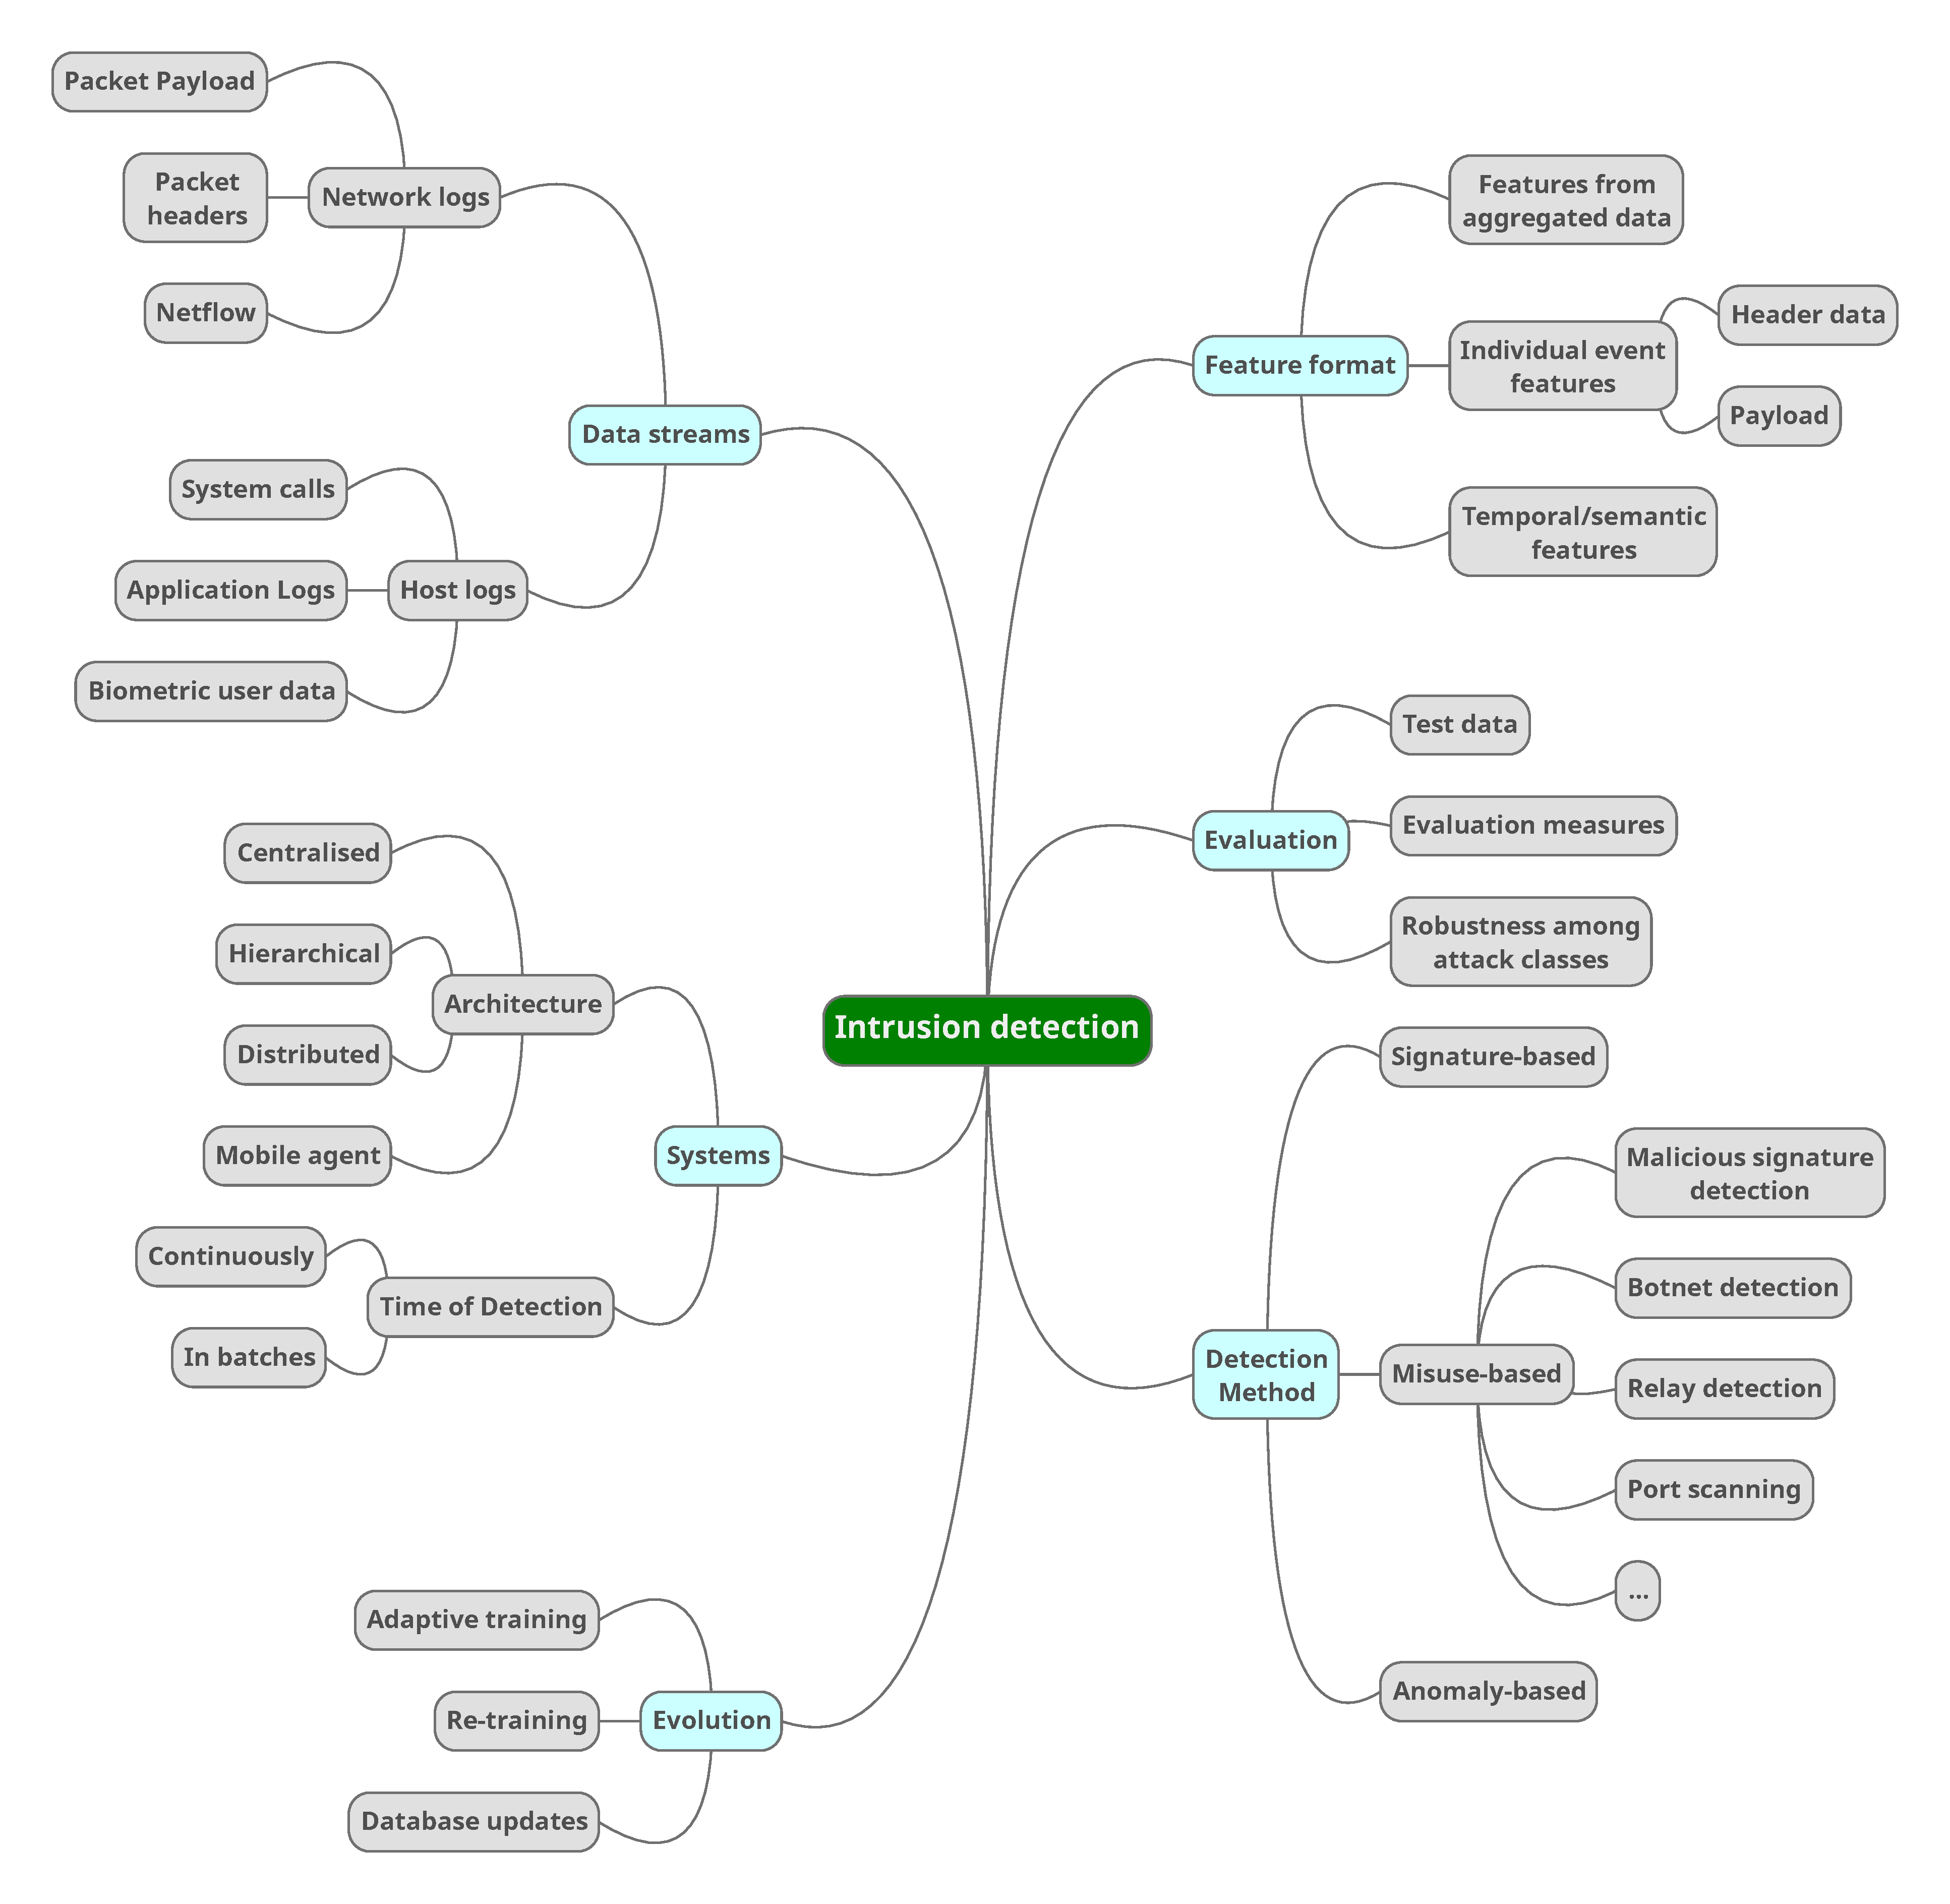
\includegraphics[scale=0.25]{Graphic2.pdf}
\caption{A broad overview over different aspects in an IDS}
\end{figure}

Host-based systems have the advantage of working with high quality data that   are   typically   very   informative \cite{lazarevic2005intrusion}. NIDS have the advantage of being plattform independent and more resiliant to attacks as detection of an infection is not done on the infected system. In this review, I will focus on work done in the area of network intrusion detection.





\subsubsection*{Architecture}

The architecture of an IDS can affect its overall performance, and is therefore an important design aspect in the operational deployment of IDSs. The decentralised topology of computer networks usually means that data is collected from multiple sensors or hosts across the network. The processing of the collecting can be done in three different ways:

Centralised IDSs gather all collected data to a central processing unit,  where  the 
analysis of the collected data and the detection take place. This unit then has complete information about the network, however the lack of scalability makes these systems less common. 

Decentralised systems follow a hierarchical structure. Sensors sent data to the closest processing unit, which pre-processes the data before sending it to the main processing unit. This way, workload is reduced at the central unit, and
the scalability problems can be avoided, but not fully overcome. 

Distributed IDS consist of multiple autonomous units that process incoming data. Processing and evaluation for malicious activity are done independently from a main unit. Individual units can communicate with each other to identify network-wide anomalies.


\subsubsection*{Detection methods}

Detection methods are the core of an IDS, and are therefore the most important design choice. Traditionally, two broad types of detection approaches are identified: a) Misuse detection and b) anomaly detection. 

Misuse detection aims at detecting a particular and well known reoccurring characteristic or pattern of a malicious behaviour. Two simple examples of such a characteristic are the large number of SYN packets sent by a host in a DoS attack, and the synchronised connection of many hosts to one server in a botnet. In misuse detection, abnormal or malicious behaviour is therefore defined first before developing a model to distinguish the defined behaviour from other traffic.

In contrast, anomaly detection aims at building a model of normal system behaviour that is accurate enough to spot any malicious behaviour as traffic that deviates from the estimated model. Anomaly detection is principally more difficult than misuse detection since the traffic model has to incorporate potentially very heterogenuous traffic behaviours. However, it is generally acknowledged that anomaly detectionhas is more suitable to detect new and previously unseen malicious behaviour as it makes no definite assumptions on the anomalous behaviour. Misuse detection is robust against evolution of malware as long as defined malicious behaviours do not change.

In reality, anomaly and misuse detection are not necessarily mutually exclusive, and there is a fluent passage between the two. This is because many anomaly detection approaches choose a particular set of features to be modelled with a particular threat in mind. For instance, models for the number of connections of a machine are naturally suitable for detecting DoS attacks, port scans, or Worm attacks. 

As misuse detection detection methods are aimed at detecting very specific behaviour, they usually only detect one type of malicious traffic. Areas that have been researched particularly well include botnet C\&C channel detection, DoS attack detection, and port scan detection. Areas that lack a comprehensive body of research are different types of R2L and U2R attacks. These are also currently the least   detected   attack   classes \cite{nisioti2018intrusion}.

\section{Scope of this work}

As my PhD-project is aimed at developing more general methods that are capable of detecting new types malicious behaviour, this review will focus mainly on anomaly detection methods. Specifically, I will look at \textbf{anomaly-based network intrusion detection}. I will however cover some areas of misuse detection if the employed methods have a potential applications to anomaly detection methods.


I will identify different classes of feature generation from network traffic and examine the benefits and drawbacks of each class. I will then proceed to review significant methods in each of the identified classes. Additionally, I will examine existing network traffic datasets that are suitable for testing anomy-based methods, and I will also give a brief overview of existing surveys and taxonomies. I will then conclude my results and briefly discuss implications for my PhD-project.

\chapter{Data}

\section{Network traffic}\label{traffic}



Computers in a network mostly communicate with each other by sending \textit{network packets} to each other, in which the transmitted information is encapsulated. Each network packet is split into the control information, also called packet header, and the user information, called payload. The packet header contains the necessary information for the correct transmission of the packet, including the transmission protocol layer (such as TCP, UDP, or ICMP), and the source and destination IP addresses and network ports\footnote{A network port is a number that identifies which service or application is responsible for the processing of incoming packets.}. It furthermore contains error-checking fields suchs as the size of the packet and a checksum over the payload, and protocol-specific fields. 


\begin{figure}[h!]
\centering
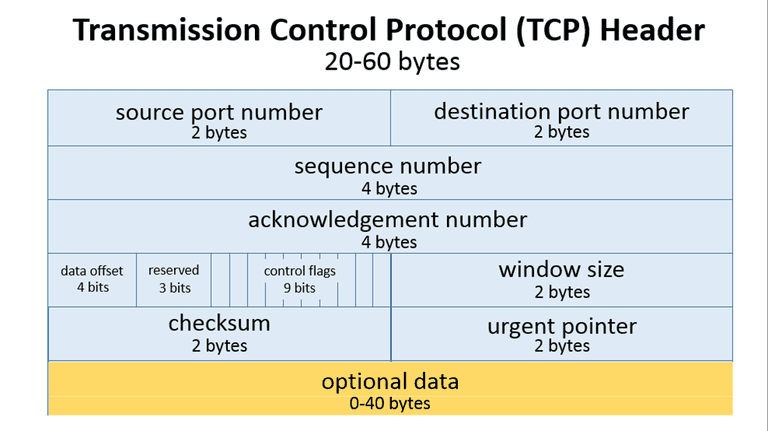
\includegraphics[scale=0.4]{tcp_header.png}
\caption{Typical format of a TCP packet. Source:\scriptsize{ https://www.lifewire.com/tcp-headers-and-udp-headers-explained-817970}\normalsize}
\end{figure}


The payload of a packet is in general the data that is carried on behalf of an application. It can be of variable length, however, it cannot exceed the maximum packet length set by the network protocol. In contrast to the packet header, the payload can be encrypted, a technique that makes it unreadable to any third parties and that is becoming increasingly common in modern computer networks. 


While traversing between to parties, a network packet can pass multiple connecting devices which direct the packet in the right direction. Any device in the immediate circuit traversed by a packet can capture and store it. In a monitoring setting, packets are usually captured by network routers and stored in the widespread \textit{pcap} format. In case of space shortage or privacy concerns, the payload of a packet can be dropped in the saving process.


Another more structured way of capturing network traffic is based on connection summaries, or \textbf{network flows}. RFC 3697 \cite{brownlee1999traffic} defines a network flow as a sequence of packets that share the same source and destination IP address, IP protocol, and for TCP and UDP connections the same source and destination port. A network flow is usually saved containing these informations along with the start and duration of the connection and the number of packets and bytes transferred in the connection.


\begin{figure}[h!]
\scriptsize
\centering
\begin{verbatim}
 Date flow start        Duration Proto  Src IP Addr:Port      Dst IP Addr:Port   Packets  Bytes Flows
 2010-09-01 00:00:00.459   0.000 UDP    127.0.0.1:24920   ->  192.168.0.1:22126      1     46     1
 2010-09-01 00:00:00.363   0.000 UDP    192.168.0.1:22126 ->  127.0.0.1:24920        1     80     1
\end{verbatim}
\normalsize
\caption{A typical network flow output}
\end{figure}


Raw packets grant full information about the connection, but take a lot of space when stored, whereas network flows give a more structured and lightweight overview over the traffic in a network. Both data formats are used widely by NIDSs.

\section{Existing datasets}

In order to evaluate their ability to model the behaviour of a network and to identify malicious activity and network intrusions, new methodologies have to be tested using existing datasets of network traffic. This network should ideally contain realistic and representative benign network traffic as well as a variety of different network intrusions. However, as  network traffic contains a vast amount of information about a network and its users, it is notoriously difficult to release a comprehensive dataset without infringing the privacy rights of the network users. 
Furthermore, the identification of malicious traffic in network traces is not straightforward and often requires a significant amount of manual labelling work.
For that reason, only a handfull of datasets for network intrusion datasets containing real world traffic exist. There have also been some efforts to artificially creating such datasets and thus bypassing any privacy concerns. However, up to today, no artificial dataset truly resembles real network traffic in every aspect \cite{nisioti2018intrusion}.

As described in a recent survey by \textbf{Ahmed et al.} \cite{ahmed2016survey}, we can generally distinguish four different types of datassets containing network traffic:

\begin{enumerate}

\item \textbf{Real network data containing known intrusions}: 

\item \textbf{Real network data containing injected intrusions}:

\item \textbf{Real network data containing no intrusions/untruthed real network data}:

\item \textbf{Synthetic network data with/without injected intrusions}:

\end{enumerate}

I will now describe the properties of existing datasets suitable for network intrusion detection. As this review is primarily concerned with anomaly detection models that require benign network traffic, I did not include datasets such as honeypots that mostly contain malicious traffic. A description that includes such datasets can be found in the below described survey by Ahmed et al. \cite{ahmed2016survey}.



\subsubsection*{Los Alamos National Laboratory, 2015 - Comprehensive, Multi-Source Cyber-Security Events \cite{akent-2015-enterprise-data}\cite{kent-2015-cyberdata1}}

In 2015, the Los Alamos National Laboratory (LANL) released a large dataset containing \textbf{network flow} traffic from teir corporate computer network, which contains about 17600 computers. The data was gathered over a period of 58 days with about 600 million events per day. The data only contains internal network connections, i.e. no flows going to or coming from computers outside the network are included. IPs and ports were de-identified (with the exception of the most prominent port), but are consistent throughout the data. Since the data stems exclusively from one corporate network, it can be assumed that it shows more homogeneity in the observed traffic patterns than  general network traffic.

Additionally, the dataset also contains other event sources which were recorded in parallel in order to give a more comprehensive look at the network, and could be very useful when investigating a detection approach that correlates multiple event sources. These sources include process events and authentication events from Windows-based computers and servers, and DNS lookup events from the DNS servers within the network. 

The dataset furthermore contains a labeled set of redteam events which should resemble intrusions. However, these events are not part of the network flow data and only contain information about the time of the attack and the attacked computer. These events apparently resemble remote \textit{access attacks}, are not described further and appear to be artificial or injected into the dataset. It is thus not certain how well they resemble actual network intrusions.


LANL released another dataset containing network flow traffic from their network in 2017 \cite{turcotte17}. This dataset is similar to the one from 2015, but spans over a longer period of time, 90 days. Furthermore, it contains no labeled malicious activity,  however that does not mean that the data is completely free of malicious activity.

\subsubsection*{CTU 2013 \cite{noauthor_ctu-13_nodate, garcia2014empirical}}

The \textit{Stratosphere Laboratory} in Prague released this dataset in 2013 to study botnet detection. It consists of more than 10 million labeled \textbf{network flows} captured on lab machines for 13 different botnet attack scenarios. Additionally, the raw packets for the botnet activity is also available for attack analysis. 

The labelling in this dataset is different from other datasets as each  flow  in  the  list  is  labeled  based  on  the  source  IP  address.  In  the experiments,  certain  hosts  are  infected  with  a  botnet  and  any  traffic  arising from such a host is labeled as Botnet traffic. Traffic from uninfected hosts is labeled as Normal. All other traffic is Background, as one cannot classify it. 

A criticism of this dataset is the unrealistically high amount of malicious traffic contained in the dataset, which makes it easier to spot it while reducing false positives. Furthermore, the way normal or background traffic is generated is described only poorly and leaves the question how representative it is of actual network traffic.

\subsubsection*{UGR 2016 \cite{macia2018ugr}}

The UGR'16 dataset was released by the University of Grenada and contains \textbf{network flow}\footnote{netflow v9} data from a spanish 3-tier ISP. This ISP is a cloud service provider to a number of companies, and thus the data comes from a much less structured network than the LANL data. It contains both client's access to the Internet and traffic from servers hosting a number of services. The data therefore contains a very wide variety of traffic patterns, an advantage emphasised by the authors. IP-adresses are consistently anonymised while network ports are unchanged. However, it is not ensured that the traffic capture is complete, i.e. that all traffic coming from and going to a particular machine is captured.

A main focus in the creation of the data was the consideration of long-term traffic evolution and observable periodicity in order to enable the testing of so called \textit{cyclostationary} traffic models. The dataset correspondingly covers a very long period, spanning from March to August of 2016, and containing about 14 GB of traffic per week. 

The data is split into a training set and a test set, with the latter containing labeled attack data. This attack data does not stem from rogue agents but is in part generated in controlled attacks on victim machines, and in part injected from previously observed malware infections. The attack data is therefore does not truly correspond to actual attacks, but achieves a high degree of similarity. The implemented attacks contain:
\begin{itemize}
\item DoS attacks (controlled attacks),
\item Port scanning (controlled attacks),
\item C\&C traffic from a botnet (injected).
\end{itemize}

The authors also acknowledge that the background traffic is not necessarily free from further attacks. In fact, three real attacks have been observed and labeled, corresponding to IP-scanning and a spam mail campaign.

\subsubsection*{UNSW-NB 2015 \cite{moustafa_unsw-nb15:_2015}}

The dataset realeased by the \textit{University of New South Wales} in 2015 contains real background traffic and synthetic attack traffic collected at the "Cyber Range Lab of the Australian Centre for Cyber Security". The data is collected from a small number of computers which generate real background traffic, and is overlayed with attack traffic using the \textit{IXIA PerfectStorm tool}. The time span of the collection is in total 31 hours.

An advantage of the collected dataset is the inclusion of both \textbf{raw packets} and \textbf{network flows} along with two other data formats containing newly engineered features. This allows a more detailed analysis of the data and possibly a better distinction between attack and benign traffic. In total, the data contains 260 000 events.

Another advantage of the data is the variety of attack data, containing a number of DoS, reconnaissance, and access attacks. However, due to the synthetical injection of these attacks, it is unclear how close they are to real-world attack scenarios.

Since this dataset is collected from a relatively small number of machines and during a limited period of time, it is furthermore unclear how suitable for capturing both the temporal evolution and the heterogeneity of real background traffic.

\subsubsection*{CICIDS 2017 \cite{gharib2016evaluation}\cite{sharafaldin2018towards}}

This dataset, released by the \textit{Canadian Institute for Cybersecurity} (CIC), contains 5 days of network traffic from 12 computers. These computers all have either different different operating systems such as Windows, OSX, or Ubuntu, or different versions of the same operating system in order to enable a wider range of attack scenarios. The network  furthermore contains switches, routers, a web server, a modem, and a firewall in order to ensure a realistic network topology. The traffic data itself consists of \textbf{labeled benign and attack traffic}, and is available as 11 GB per day of \textbf{raw packets} with payloads, or as \textbf{network flows}. 

It was ensured that the data contains all traffic coming and going from individual machines. However, in contrast to other datasets, the background traffic is not directly generated through user interactions on the machine, but by using a method to profile abstract user behaviour in different traffic protocol. The purpose of this is to make the traffic more heterogenuous and to ensure that different types of behaviour are present in the data during the comparably short time span. This  However, it is not completely clear how much of the underlying structure of real traffic is lost in the process, and therefore how suitable this data is to build models of benign user activity.

The attack data of this dataset is one of the most diverse among NID datasets, as it contains a variety of up-to-date attacks, such as different types of DoS attacks, SQL-injections and Heart-bleed attack, network scanning, or botnet activity. These are not always successful in order to reflect actual attack scenarios. However, the authors did not describe very well how the data from these attacks is generated and combined with the background traffic as it is also processed through a form of profiling engine. 

The CIC released another very similar dataset to this one in 2012.

\subsubsection*{DARPA 1998 \cite{lippmann2000evaluating}}

The \textit{Defense Advanced Research Projects Agency} released the first major dataset to test network intrusion detection systems. The data stems from two experiments at the \textit{MIT Lincoln Laboratory} were multiple victim hosts running Unix and Windows NT were subject of over 200 attacks of 58 different types. The data spans three weeks of training and two weeks of testing data and contains \textit{raw packets} that are labeled. It was since then heavily used as a benchmark to test new detection methods. %In 2000, the original data was post-processed to reduce some of its shortcomings.

Also due to its prominence, it was heavily scrutinised and received a lot of criticism for its lack of realistic background traffic, which was generated through simulation procedure, and the presence of artifacts from these simulations in the data that could heavily skew any model relying on benign traffic. Also, the high percentage of attack traffic in the data is described as unrealistic.

Furthermore, since the dataset is now more than 20 years old, it is remarked that both the benign and attack traffic does not resemble modern network traffic anymore. 

\subsubsection*{KDD Cup 1999 \cite{cup1999data,cup1999dataset}/NSL-KDD 2012 \cite{tavallaee2012nsl}}

The \textit{MIT Lincoln Laboratory} created this dataset in 1999 by processing portions of the 1998 DARPA dataset with new labels for a competition at the conference on \textit{Knowledge Discovery and Data Mining}, and is the most widely used dataset in intrusion detection. It contains 2 million connections summaries in a new format and in total 38 attack types. This new format is essentially a form of \textbf{network flows} with a greatly increased number of features, 46 in total, which give additional details about the origin of the connection. The availability of these features in a real-world application however is in my opinion unrealistic as most of them could be mined due to the availability of parallel surveilance of the host, a Solaris-based system. However, we can see significant differences in today's operating systems which barely resemble Solaris. In addition, parallel host system surveilance usually cannot be taken for granted in a realistic network environment. Naturally, as the KDD'99 data stems directly from the DARPA dataset, it also faces the same problems and criticism. 

The \textit{Canadian Institute for Cybersecurity} postprocessed the KDD'99 data in order to address some of its shortcomings. This includes removing redundant records, balancing the size of the training and test data, and adjusting the proportion of attack traffic in the data. However, the biggest criticism from the KDD'99 and the DARPA data, the unrealistic generation of background data, still prevails.

\subsubsection*{LBNL 2013 \cite{pang2005first}}

This dataset released by the \textit{Lawrence Berkeley National Laboratory} in 2005 is the first one to examine internal network traffic inside a modern enterprise. It contains more than 100 hours of \textit{packet headers} from several thousand internal hosts. 

This dataset contains no known attack traffic, and is therefore only suitable for traffic analysis and model fitting analysis. Furthermore, as being the first dataset containing enterprise traffic, privacy concerns caused the authors to remove any possibilities to identify individual IP addresses.

In 2011, Saad et al. \cite{saad2011detecting} combined this dataset with existing botnet traffic to create a dataset containing both benign and attack traffic. 

\subsubsection*{UNIBS 2009\cite{UNIBS2009data}}

This dataset was collected on the campus network of the \textit{University of Brescia} on three consecutive days in 2009. The dataset contains in total 79000 anonymised TCP and UDP \textit{network flows}. 

This dataset is not directed towards intrusion detection research, but was made as \textit{ground truth data} for traffic classification. It therefore contains labels which indicate which of in total six applications generated the corresponding traffic flow. It might however still be of interest for model assessment in intrusion detection that is relying on traffic classification.

\subsubsection*{CAIDA 2016 \cite{walsworth2015caida}}

The \textit{Center for Applied Internet Data Analysis} started collecting network traces from a high-speed backbone link in 2008 with the collection still ongoing. The data is available in anonymised yearly datasets containing one hour of \textbf{packet headers} for each month. 

Since the traffic is collected from a backbone link, it is very unstructured and heterogenuous. It is furthermore not necessarily free from attack traffic. Although this dataset has been used for intrusion detection before, it is more suitable for general internet traffic analysis.


\subsubsection*{MAWI 2000 \cite{sony2000traffic}}



Similarly to the CAIDA dataset, this dataset contains \textbf{packet headers} from the WIDE backbone. It is therefore similarly unstructured, anonymised, and not free from attack traffic. Since this dataset was already collected and released in 2000, it can also be remarked that the contained traffic is too old to represent modern traffic. 

\subsubsection*{ADFA 2013/2014 \cite{creech2014developing,creech2013generation}}

The ADFA datasets, released by the \textit{University of New South Wales}, focuses on attack scenarios on Linux and Windows systems as well as \textbf{stealth attacks}. To create host targets, the authors  installed web servers and database servers , which were then subject to a number of attacks. 

The dataset contains both attack traffic and benign traffic. However, the dataset is directed more towards attack scenario analysis and is criticised as being unsuitable for intrusion detection due to its lack of traffic diversity. Furthermore, the attack traffic is not well separated from the normal one.

\subsubsection*{ICT datasets \cite{USC2010ICT}}

The \textit{Impact Cyber Trust} releases cyber security oriented data. Its repository includes many datasets, synthetic as well as real captures, from different sources. Many datasets focus on observed attack data and thus are not directly applicable to intrusion detection. Furthermore, there is in general very little information provided that describes a dataset's origin, which makes it hard to investigate the network topology.

Among the more useful datasets are the \textit{USC datasets}\footnote{DS-062, LANDER Data, and DS-266}, which contain network traffic (both \textbf{packet headers} and \textbf{network flows}) from academic networks in the US between 2008 and 2010. The datasets are very large, with the largest one covering 48 hours and containing 357 GB of packet headers. 


\chapter{Methods and Systems for Network Anomaly Detection}\label{Anomaly detection}

\section{Feature generation}

Anomaly-based intrusion detection moved into the focus of researchers at the end of the 1990s, with many advances and new ideas being implemented between 1998 and 2005. Anomaly detection methods often rely heavily on tools from the area of machine learning and statistics in order to generate quantitative models for normal traffic from large amounts of data. A challenge for researchers is that network traffic data, both in the form of packet headers or network flows, is a mix of continuous and categorical variables, with the latter often having an immense number of categories. Furthermore, the data has a temporal aspect, which is however only incorporated by a few authors. 

Many existing surveys \cite{ahmed2016survey,buczak_survey_2016,bhuyan_network_2014} distinguish anomaly-based approaches directly according to the area the method is borrowed from, e.g. into statistical, supervised, unsupervised methods and so forth. 
However, this neglects an aspect that should be the primary decision factor for which method or model to use: Feature engineering. As network traffic is itself not a data format, it is necessary to generate meaningful features from it. The type of features is crucial for accurateness of traffic representation and ultimately for the types of malicious activity that can be discovered. 


While surveying existing literature, I identified four different classes of detection methods, depending on how the authors incorporate traffic features: 

\begin{itemize}
\item Traffic aggregation-based methods,
\item event-based methods,
\item and methods that incorporate the temporal structure of network events.
\end{itemize}

Iwill now explain the nature of the different classes and analyse anomaly-based methods in each class. It is important to mention that I neglected methods that are based on \textbf{payload inspection}, which form themselves another class of detection methods. However, payload-based methods are dependent on unencrypted traffic and are often seen as to computationally expensive for a successfull deployment in real networks. As encryption becomes more and more the standard in the way we communicate over the internet, I will not discuss payload-based methods in this work and instead generally assume that no unencrypted traffic is available for my PhD-project.

\section{Approaches based on Volume or Traffic Aggregation}

Traffic aggregation is a simple way of creating a contextual format of network traffic in contrast to isolated events. Usually, all events in a certain time interval are binned and summary statistics over the different traffic parameters are calculated, such as the sum of events of bytes transferred, or the number of distinct IP addresses/ports communicating. Events in each time interval therefore stand in a contextual relationship as they together influence the different summary statistics.  Aggregation of traffic can be done for individual hosts as well as for groups or entire networks, while the computational load depends on the choice of summary statistics. 

Methods relying on traffic aggregation are most suitable for attacks in which events form a collective instead of a point anomaly. Examples  of attacks forming collective anomalies are DoS and port scanning attacks as events like a half-open connection are not anomalous themselves, but are anomalous when occurring in larger numbers. Attacks that contain less volume however are less likely to be detected in aggregated traffic as individual features of the events would have to be large or unusual enough to influence the summary statistic of the entire group.


\subsection{Subspace projection/PCA-based}

\textit{Principal Component Analysis} is a statistical form of \textit{orthogonal coordinate transformation} to convert a set of observations (or feature vectors) into a set of linearly independent variables\footnote{the \textit{principal components}}. These variables uncorrelated variables each account for differing amounts of the variation contained in the data. By projecting an observation only onto the components that account for the most variation, it is possible to retain most of the information while operating in much lower dimensions.

\textbf{Lakhina et al.} \cite{lakhina_diagnosing_2004,lakhina_characterization_2004}  introduced a PCA-based anomaly detection method for network traffic in 2004. In their approach, they aggregated the network flows for each OD\footnote{Origin-Destination} pair into 5-minute bins, with the number of transferred bytes, packets, and flows being the features for each bin. Each 120 consecutive bins were then treated as a an observation (with $3\cdot 120$ variables), and PCA was then applied to the collection of observations. The first $5$ principal components are then identified as the dominant temporal patterns. Anomalies were then identified as observations that could only very poorly reconstructed using the first $5$ principle components. Since then, this approach has been adopted to several other datasets without much methodological advances. Camacho et al. \cite{camacho_pca-based_2016} proposed an improvement to the existing PCA-based approach with a more natural implementation of spotting anomalies. 

This approach can be applied to individual OD pairs, or on a network-wide basis by using q-statistics to spot multivariate anomalies. The approach was tested on data from the Abilene backbone network, and worked well to identify significant episodes such as DoS attacks, fast spreading worms and other large-scale scanning activity, alpha-flows, or power outages. 

Naturally, since the traffic is aggregated into bins and the temporal behaviour of these bins are examined, this approach is aimed towards identifying attacks with a comparably large volume of traffic, even if they are isolated in time. It is however unlikely that it is capable of spotting smaller U2R and R2L attacks or C\&C traffic. Another possible criticism is that anomalies are not spotted immediately, but in the worst case after hours.


\textbf{Ringberg and Rexford} \cite{ringberg_sensitivity_2007} provided a discussion of PCA-based approaches to traffic anomaly detection. They concluded that PCA is very sensitive to small differences in the number of used principal components and to the level of aggregation of the traffic measurements. Furthermore, the training data has to be absolutely free of any traffic anomalies, otherwise the projection onto the first principle components can change drastically. 

\subsection{Entropy-based}

The entropy is a measure for the degree of disorder a system is in. Applied to network traffic, a popular quantity to measure is the dispersion of events onto different source or destination IP addresses. A high entropy would correspond to all events being evenly distributed among the all existing IPs while a low entropy corresponds to the majority of events being concentrated between a small number of IPs.  Entropy-based approaches are usually emplyed more in misuse detection, but can also have reasonable applications in anomaly detection.

\textbf{Wagner and Plattner} \cite{wagner2005entropy} measured the entropy of network flow distribution across source and destination IP addresses and across source and destination ports on a network-wide basis. The entropy is measured in a sliding window of 5-minutes with 1-minute shifts and monitored continuously. Anomalies are flagged as sudden changes in one or more of the mentioned entropy sources with tresholds that were determined from empirical judgement. The described measures were applied to network data from a swiss internet backbone which contained data from two large-scale worm outbreaks\footnote{\textit{Blaster worm} and \textit{Witty worm}, both more than 50 000 infections}. The characteristics of these worms in terms of entropy changes\footnote{Source IP and destination port entropy decreases drastically, destination IP entropy increases moderately} were then analysed as an evaluation of the technique.

\textbf{Lakhina et al.} \cite{lakhina2005mining} used entropy in a similar, albeit more sophisticated way to detect anomalies. Instead of using entropy on a network-wide basis, it used to monitor src and dst IP and port distributions on individual hosts over time. The obtained values are then bundled in a three-way matrix $H(t,p,k)$ where $t$ is the current time, $p$ is the particular host, and $k$ is one of the four monitored traffic features. This data matrix is then converted into a two-way matrix and similar to other work by Lakhina, a PCA-like subspace projection is applied to mine temporal features as orthogonal components. However, here these components reflect correlations in simultaneous entropy changes on different hosts and features. Anomalies are again detected as poor reconstructions by via the most dominant components, and the performance is examined using untruthed data from the Abilene backbone network. Another clever addition of this paper is the use of unsupervised learning to identify different types of observed anomalies. This is done by applying hierarchichal clustering with a fixed number of clusters to the residual vector of $H$. However, contains some obvious flaws that in my opinion prevent a generalised grouping of anomalies.


\subsection{Wavelet-based}

Wavelet modelling is a frequency-based signal processing approach. Amplitudes of most signals can be described as a finite sum of wavelets with different frequencies. These frequency coefficients can then be used as a measure to describe the signal's generalised behaviour, and to compare with future data from the same signal. Three significant papers applying wavelet modelling to intrusion detection can be found:

%\subsubsection*{Barford et al. - A Signal Analysis of Network Traffic Anomalies, 2002}

Both \textbf{Barford et al.} \cite{barford2002signal}, and \textbf{Thottan and Ji} \cite{thottan2003anomaly} introduced wavelets to network anomaly detection in 2002/2003. Both approaches are fairly simple, as they only look at the network flow numbers from multiple machines at different points in the network, aggregated into 5-minute intervals. Using enough anomaly-free training data\footnote{It is crucial that this data is absolutely free of anomalies that are to be detected}, this volume signal can be described by a set of frequency-components. Barford et al. then compare the frequencies of any future traffic episodes against this set, and marked as anomalous if a treshold is exceed. The approach is directed towards detecting network-wide flash crowds, DoS attacks, and outages, which is evaluated using proprietary data. Thottan and Ji detected anomalies by looking at the reconstruction error of such traffic episodes using the estimated frequency-components instead comparing different estimates. The reconstruction error is assumed to follow a gaussian distribution, and anomalies can be detected using a hypothesis test.

\textbf{Jian et al.} \cite{jiang2014transform} proposed a refined wavelet-based model in 2014 which is applied to individual OD pairs. All observed OD pairs in the network are grouped into $q$\footnote{number depends on network topology} groups. To each group, an S-transformation (a modified version of a wavelet-transformion) is applied. The signal for each OD pair is then reconstructed using only the estimates of the high-frequency components since these correspond to any bursty behaviour. Now, the reconstructed signal is free from any slow variation and contains only fast and bursty behaviour. The assumption of the authors this degenerated signal must be heavily correlated between individual OD pairs. Using a sliding window, the pairwise correlations of each OD pair is computed. If the correlation for any pair falls below a certain treshold, this pair is marked as an anomaly. The approach is designed to detect volume-intensive attacks on busy servers, the exact motivation for this approach however is not described very well by the authors. The evaluation is done using data from the \textit{Abilene backbone}.

It is clear that any approach that looks exclusively at the traffic volume either between individual hosts or in a network-wide fashion will only detect attacks with sufficient attack volume, such as DoS attacks. Additionally, wavelet-based approaches do not provide a probabilistic framework for anomaly detection, which makes the seperation of true anomalies from false positives difficult, especially in larger networks. 


\subsection{Other}

\textbf{Kind et al.} \cite{kind2009histogram} proposed a network-wide detection approach that is based on traffic histograms and clustering to identify and model substructures in normal traffic for better anomaly detection. A number of different traffic quantities are divided into a fixed number of subgroups, such intervals of IP-addresses or network ports, bins of packet sizes or connection durations, or the different TCP flags in a connection. For every different feature, authors create histograms measuring the number of events occuring in each subgroup during a 5-minute interval. Histograms are monitored over a period of time without any malicious activity in order to gather a collection of training histograms. After removing subgroups that remain, each traffic feature is then divided into clusters using the Mahalanobis-distance measure as a similarity metric between histograms and either hierarchical or $k$-means clustering. Anomalies in individual traffic features can then be detected as histograms with distances from the nearest cluster that exceed a certain treshold. Evaluation is conducted with an unnamed dataset containing 15 labeled attack, containing DoS attacks, worm propagation and network scanning, and network-wide system fingerprinting, and mail bombs, of which 13 were detected. Unsurprisingly, the two undetected attacks addressed fewer machines and thus consisted of less traffic. In general, this approach indivates a great improvement from the previous approaches as it is the first significant attempt at discovering substructures in aggregated traffic, which generally grants a better detection of non-trivial anomalies. An interesting improvement would be to correlate simultaneous outliers in different features using a variant of hypothesis tests as a lower anomaly treshold could be used.

\textbf{Heard et al.} \cite{heard2016network, heard2016topic} recently proposed a rather different approach: The authors here monitor the number of network-internal connections and authentication events on each machine over 5-minute invervals. The authors observed network-wide a strong \textit{power-law-like} distributions of the number of events per host, i.e. the number of events is very large for some hosts an declines proportional to $c x^{-k}$ where $x$ is the number of the host. The authors then model the behaviour using two related probabilistic methods, the \textit{Dirichlet process} and \textit{latent Dirichlet allocation}, where the model parameters were estimated from attack-free training data in a Bayesian fashion. Event numbers which deviate strongly from the estimated model were then scored according to their unlikeliness. Both approaches were tested using the LANL dataset and asigned high scores to known inected computers. Furthermore, the authors claim to have possibly detected an unlabeled machine as being infected through manual investigation after it was asigned the highest score of all machines. As this approach is solely looking at the number of incoming and outgoing connections and events, this approach similarly to many entropy-based approaches covers a narrow area of possible malicious activity, and it is concerning that the ratio of benign machines with high anomaly scores (which can be seen as false alerts) is very high. However, this approach marks a step into a more probabilistic anomaly asignement which is beneficial for a more adaptive approach to model estimation and a quantification of detection certainty.





\section{Event-based}

The majority of network anomaly detection approaches are based on point anomaly detection, in other word they identify individual events as malicious solely on the observed characteristics of this event. Such events are usually either individual network packets or flows. In contrast to approaches on aggregated traffic, which can usually only detect attacks with a certain traffic volume, an event-based approach is independent of the traffic volume and therefore more suitable to identify activities consisting of only a few events, such as data exfiltration, R2L attacks, or C\&C communication.

\subsection{Statistics-based}

%\subsubsection*{Mahoney and Chan - Learning Nonstationary Models of Normal Network Traffic for Novel Attacks, 2002 \cite{mahoney2002learning}}

\textbf{Mahoney and Chen} \cite{mahoney2002learning} were one of the first to develop statistical methods to identify anomalous events in network traffic. Their approach consists of two separate scoring stages.

The first stage is the \textit{packet header anomaly detection} (PHAD). Here, the 33 different fields of an Ethernet-transmitted packet are converted from their one to four bytes to an integer value. The gathered values for each field are then clustered in a simple agglomerative fashion, and the clusters are updated each time a new packet arrives in order to keep the number of clusters below a treshold. The anomaly score of a packet is then proportional to the number of fields in which the clusters had to be updated. 

At the second stage, the \textit{application layer anomaly detection} (ALAD), scores are asigned to the packet according to a frequency table build using previously collected packets. These frequency tables address the several combinations of a variable conditional on another variable. These variables include source or destination IPs, destination port, TCP flags, or the first word of the payload. An interesting factor considered by the authors is the inclusion of the time since last observance for each of these frequency tables in the anomaly score.

The approach was tested on the DARPA'98 dataset and detected 70 out of 180 attacks while raising 100 false alerts. When the unrealistically high number of malicious packets in the data is considered, the number of false alerts is alarmingly high. Another issue with this publication is that the authors claim that they are building nonstationary models, yet give little how these models should adapt over time. 

%\subsubsection*{Kruegel et al., Service Specific Anomaly Detection for Network Intrusion Detection, 2002 \cite{krugel2002service}}

\textbf{Kruegel et al.} \cite{krugel2002service} developed an approach that is aimed fitting individual models for each of the different services generating network traffic. Their assumption is that by concentrating on only one type of traffic, statistical data with lesser variance can be collected. 

The approach works as following: Once a connection is openened, the packet processing unit reads the first packets of a connection and extracts the specific service, such as a get request for a HTTP request. It is then asigned an anomaly score based on the different aspects: The type of service, the length of the request, and the payload contained in the request. 

The anomaly score associated with the type of service is proportional to the negative logarithm of the service frequency observed in the training data. Thus, rare services receive a higher anomaly score. 

To score the length $l$ of the request, the mean $\mu$ and standard deviations $\sigma$ of request lengths in the training data is estimated using maximum likelihood. The score is then proportional to $(l-\mu)/\sigma$.

Finally, the payload is scored according to a frequency distribution of the letters occuring in the training data. The deviation of a payload from the distribution can easily be estimated using a $\chi^2$ test. By scoring the payload of a service request, the authors hope to detect malicious requests that try to disrupt the reciver through a corrupt combination of non-printable or replaced characters. Kruegel et al. \cite{kruegel2005multi} later greatly improved the payload scoring specifically for HTTP traffic by using a \textit{Markov model}.


In their evaluation, the authors only considered DNS traffic due to lack of resources and space. Testing was done after a calibration of the anomaly tresholds by attacking their own DNS servers with 5 different attacks, all of which have been detected. However, evaluation of other services and on independent data would shed more light on the actual performance. Another important issue not addressed by the authors is the possible temporal drift of the estimated distributions.



\textbf{Both} of these papers introduced introduced new concepts of how to model the distributions of individual event features which take into account the nature of network traffic. However, there is a lot to criticise about these approaches. The developed estimation and scoring methods lack a broader probabilistic foundation and can be improved greatly. Furthermore, these papers do not address any possible interdependence of features, which could lead to serious mismodelling of behaviour observed as anomalous. Also, it is unclear if these models will provide behaviour over time.


\subsection{Classifier-based}

Due to the availability of datasets such as DARPA'98 or KDD'99 which are labeled and rich in both benign and malicious traffic, it is tempting to apply existing machine learning approaches directly onto the event features provided in the data. Additionally, the KDD'99 data contains significantly more features for each event than normal network flow data. Consequently, there exists a large body of literature drawing from this apparent opportunity and applying a variety of classifiers such as  decision trees, support vector machines, Na\"ive Bayes, or Neural Networks to these two datasets. However, such approaches often lack a greater understanding of the utilised data and the overall problem of intrusion detection, and achieved test results can normally not translated into good performance in realistic environments. Also, even if labels for both normal and anomalous data is available, the imbalance of normal traffic to malicious one generally makes learning a classifier hard.

Two illustrative examples are the works of \textbf{Barbar\'a et al.} \cite{barbara2001detecting} on the DARPA 98 data, and of \textbf{Javaid et al.} \cite{javaid2016deep} on the NSL-KDD data, both highly cited papers. Barba\'a et al. apply a Bayesian network classifier on the available features\footnote{Numerical features and dictionaries of pre-seen IPs and ports} of individual packets while Javaid et al. train two layers of neural networks on the numerical features of the KDD flow events. Both approaches achieve high detection accuracies on the used data. The overall assumption here is that the classifier can generalise the learned differences that separate benign from malicious traffic in the dataset to a broader set of malware classes or even most of them. 

However, there is no valid reason to assume that this is true. I would instead argue against it and claim that since there are only a relatively small number of different malware activity in every available dataset, the malicious traffic in a dataset only contains very little variation, which makes it fairly easy to overfit the malicious traffic with the available features and achieve high detection accuracy. %\footnote{since the training and test data is not separated with regards to different malware classes}. 
This is especially true for the DARPA and the KDD data as they contain artifacts and  duplicate entries, which are known lead to over-estimation of anomaly detection performance, according to recent work by \textbf{Ahmed and Mahmood} \cite{ahmed2016survey}. Another important point is that benign traffic is very heterogenous, and a classifier would have to be trained for every network to learn how to separate it from malicious traffic. Truthed data containing both attack and benign traffic is however very rare and notoriously hard to get, so it is far from realistic to assume that such data is available for every network. It is also important to repeat that event data is generally not as rich in features as the KDD data, which will further impact the ability of detecting malware. 


Other notable examples can be found in the references \cite{gupta_layered_2010,muda_intrusion_2011,maglaras_intrusion_2014,
peddabachigari_intrusion_nodate,ramos_antids_2005}.
An interesting contribution was made by \textbf{Hu et al.} \cite{hu2014online}. While having the same methodological flaws described above, the paper is more noteworthy for the proposal of a distributed learning framework that allows the large-scale training of a host-based model on many machines simultaneously.

\subsection{Clustering based}

Clustering is a techniques designed to identify and parametrise areas of higher probability density in the feature space of a dataset and can thus discover underlying structures in unlabelled data. These areas are identified as cumulations of datapoints that lie close to each other according to a distance metric. This can be very helpful in building an anomaly detection framework as it less trivial anomalies can be detected as datapoints outside of the identified data structure. 

Clustering overcomes many drawbacks that other machine learning techniques face in the area of intrusion detection: As it does not perform a classification task, it is better suited to deal with unlabelled data that has a high imbalance between two classes, in our case normal and malicious traffic. Clustering furthermore usually has a low testing time and can be used for network data that does not labelled attack data. Robust techniques that can identify the existence of anomalies in the training data exist, however it is not properly tested how well translates to spotting malicious traffic. A drawback of clustering techniques are that only numerical variables can be used as input as a distance measure cannot be asigned to categorical variables.


Similarly to classification-based methods, the availability of the DARPA'98 and the KDD'99 dataset make the direct application of clustering techniques to raw data as an anomaly detection technique or as a pre-processing tool for classification based methods tempting. The described benefits of clustering can reduce some of the above described flaws of classification-based methods as it reduces overfitting and computation time. However, again little attention is paid to the fact that the features available in these datasets are unrealistic and flawed, and the identification rates achieved are not transferable to other datasets.

Lin et al. \cite{lin2015cann} recently developed a clustering based framework for intrusion detection, called \textit{CANN}. They apply \textit{k-means clustering} to the normalised numeric features of the KDD'99 data for $k=5$. Anomalies are then identified as points exceeding a treshold distance from these centres using a specific distance metric that includes every cluster center, comparable with the \textit{k-neirest neighbour} technique. Several other authors use clustering as a form of data pre-processing to reducing overfitting and computation time. Among them  include \textbf{Wang et al.} \cite{wang2010new} who use \textit{ant-colony based clustering} combined with a neural network classifier with mixed results, or \textbf{Giacinto et al.} \cite{giacinto2008intrusion} who used k-means clustering with a \textit{support vector machine} classifier, both on the KDD'99 data.


Clustering of network events is related to traffic classification in that different traffic generator classes which influence the observed event features are assumed to exist. As I mentioned above, raw network events such as flows are not overly rich in features and are thus limited in the amount of traffic structure they can convey. Anomaly detection techniques that rely on clustering can benefit from the data mining techniques developed in the area of traffic classification, which is why I will include some noteworthy results here. 

In 2004, \textbf{McGregor et al.} \cite{mcgregor2004flow} published one of the earliest works on network traffic clustering. They use a probabilistic method, the \textit{Gaussian mixture model} (GMM), in order to estimate the position and the width of a small number of clusters. As this approach is based on the likelihood of the datapoints in a Gaussian model, it is possible to estimate the number of clusters using GMMs, a big advantage over most other methods were the number of clusters has to be chosen manually. 

\subsubsection*{Traffic Classification and its relation to Clustering}

An important assumptions the authors make is that there can be several quite distinct classes of traffic within individual protocols, and that these classes can themselve be spread accross more than one port or protocol. The usual numeric features of network flows, the number of bytes and packets and the duration of the connection, are extended by statistics\footnote{mean, first five modes, minimum and maximum, and quartiles} of the packet sizes and the interarrival times of packets and the idle time which is the cumulated interarrival times exceeding two seconds. Furthermore, the notion of transaction and bulk mode of a connection is established, with the latter denoting more than three successive packets being sent in one direction, and the number of transitions between the two are recorded. A GMM is then trained using standard expectation maximisation, and 6 different well-separated clusters of traffic are identified and described. It is however questionable how representative 6 clusters are for the variety of network traffic, and how accurate the assumption of Gaussian distributions for such a small number of clusters is. \textit{Zander et al.} \cite{zander2005automated} in 2005 use a very similar approach with a slightly more sophisticated probabilistic clustering method. The concept of extracting packet size and interarrival statistics as additional flow features is also used in classifier-based appraoches to traffic classification, most notably \textbf{Moore et al.} \cite{auld2007bayesian,moore2005internet} with classification accuracies up to $99\%$ using a Bayesian neural network. Remarkably, accuracy only decreases to $95\%$ when testing applications eight months apart.

A slightly different approach is taken by \textbf{Bernaille et al.} \cite{bernaille2006traffic}: Instead of gathering statistics over the whole connection, only the size of the first five packets of a flow are used, and the flows are then clustered using k-means for individual protocols. The intuition here is that the first few packets capture the initial negotiating phase, which is usually a pre-defined sequence of messages with relatively consistent packet sizes. The benefit of this approach is that a flow can be classified before it ended, however out-of-order packets will lead to very different cluster asignements. The authors were able to distuingish flows from 10 different applications relatively accurately. A similar, yet classifier-based and thus supervised approach for traffic classification was developed by \textbf{Crotti et al.} \cite{crotti2007traffic}.

\textbf{Yen et al.} \cite{yen2009browser} propose a very interesting method to passively fingerprint different browser implementations. They observed that in order to speed up content retrieval, different techniques are used in different browsers, which can in part be seen by the fact that Firefox initiates more flows than the other browsers upon connecting to a website, Opera sends more packets in earlier flows, and Safari sends fewer packets overall. In order to construct a classifier, they extract similar statistics for the byte and packet counts in each flow as McGregor et al. \cite{mcgregor2004flow}. Furthermore, they use the number of simultaneously open flows and the time passed since the last start of a flow as features. Furthermore, for each retrieved website \footnote{It is however unclear, how the authors identify all flows corresponding one website retrieval in overlapping traffic}, the total number of flows along with the cumulative byte count and retrieval duration are identified as useful classification features. A SVM-classifier is then be trained using these features and a dataset of website retrievals with labels for the corresponding browser. For this, a labelled dataset was generated by the authors for four different browser\footnote{Firefox, Opera, Safari, Internet Explorer} and 150 websites over the course of multiple months. Acchieved classification accuracy is between $71\%$ and $100\%$, depending on how many websites are left unclassified due to uncertainty of the classifier. However, as this detection method is supervised and depends on timely separated website retrievals, it is unclear how well these results translate to untruthed real-world data more common in the area of anomaly detection.






\subsection{Representation-learning based}

Representation learning, also called \textit{feature learning} is a set of techniques aimed at automatically learning underlying structures in raw and noisy data, and are in a broader sense a form of density estimation. These techniques are often based on learning lower dimensional representations of the data, similar to subspace-projections, and are therefore suitable for data with highly correlated variables. Existing methods are often based on neural-networks and backpropagation. Learning of normal traffic behaviour can be done directly using representation learning instead of deriving probability distributions and correlations of individual traffic variables first. However, current methods are only suitable for numerical variables and not for categorical ones.


\textbf{Ramadas and Ostermann} \cite{ramadas2003detecting} in 2003 proposed the use of \textit{self-organizing maps} (SOM) to learn the representation of individual types of network services. A self-organizing map projects input data onto a two-dimensional lattice, which is why they are often used for data visualisation. The projection is learned using groups of competitive neurons. Each generation drops neurons which have different representations from the group, which makes this approach particularly computation-intensive. Since the projected data lies densely together, the authors train the map with normal traffic and detect anomalous events via their distance to the nearest neighbour. The authors however only evaluate their approach using 6 numerical features from DNS and HTTP network flows which they collected themselves. This makes a performance evaluation difficult and also leaves the question open how much knowledge is gained by using only 6 different flow features. Kayacik et al. \cite{kayacik2007hierarchical} later extend this approach to all 41 numerical features of the KDD'99 data. The evaluation showed most success in the detection of DoS and probing attacks.


A direct approach to outlier detection is provided by \textbf{Hawkins et al}. \cite{hawkins_outlier_2002} in 2002. They applied a \textit{replicator neural network}\footnote{Also called \textit{Autoencoder network}} to the numerical features of the KDD'99 data. A replicator network tries to accurately reconstruct any input data it receives after sending it through a lower-dimensional bottleneck. The difference to an SOM is that learning is based on error-correction. By training it on normal traffic, the authors build a model that can reconstruct any normal traffic from its lower-dimensional representation with small errors. Anomalies are then detected as input data which is not reconstructed well and therefore deviates substantially from the learned data structures. Supposedly, a replicator network is robust agains small numbers of outliers in the training data. However, it requires careful examination how well this assumption translates onto network traffic. 

\textbf{Gao et al}. \cite{gao_intrusion_2014} use a similar technique called \textit{deep belief networks} (DBN) on the KDD'99 data. They have a similar structure to replicator networks, but training is more difficult since their hidden layers are probabilistic. The authors mainly focus on explaining the benefits of using probabilistic neurons and discussing possible ways how to train a DBN on network traffic while not providing a thorough discussion of their results.

In general, effective applications of representation learning require the availability of data rich in features, something that is in general not true for network flow data. Existing approaches based on representation learning benefited heavily from the availability of additional features in the KDD'99 dataset, which sets an unrealistic standard. Representation learning can offer a great advances to the area of intrusion detection, however new approaches have to address the issue of engineering features suitable for learning real representations of the data.





\section{Temporal correlation/Semantics-based}

Despite network traffic being a stream of events, most anomaly-based intrusion detection approaches neglect any temporal features. Nevertheless, malicious behaviour most often is composed of  a series  of related computer and network  events and have a distinct temporal and semantic profile \cite{ye2000markov}. As an example, an intruder using a session relay to exfiltrate information or pass malicious code generates a strong dependency between incoming packets in one connection and outgoing packets in the other connection (and vice versa) albeit the individual packets or connections resemble perfectly benign behaviour\footnote{as they are essentially two normal connections that are relayed by the intruder}. Building a model that can that can understand relations and dependencies between individual events could potentially lead to great improvements in the detection of otherwise non-anomalous attacks. 

Since a machine's network traffic is the collective stream of multiple processes accessing the internet, individual traffic sequences are mixed with others, which makes the modelling of temporal dependencies a non-trivial task. In comparison to the other identified categories, research in the area of anomaly detection using temporal correlation or semantic models is sparse. 


In 2003, \textbf{Krishnamurthy et al.} \cite{krishnamurthy2003sketch} propose a rather simple, yet efficient method for network-wide monitoring of individual key occurrences in an online fashion. For that, a sliding window approach is used to asign all keys (which here stand for individual IP addresses or network ports) a value containing the number of its occurrency. For each key, the collected values are then used to train either an \textit{ARIMA} or a \textit{Holt-Winters} method, both popular and powerful time-series forecasting models which can be trained in an online fashion. Anomalies are then identified as values with a forecasting error exceeding a certain treshold and thus indicating a sudden change in occurrency-behaviour of that particular key. This is an improvement to summarisation measures such as entropy or histograms in two ways: It provides a better resolution of individual traffic channels, enabling the detection of attacks with far less volume, and enabling the modelling of more complex temporal patterns which become apparent on a lower level. And it makes attack attribution far simpler by indicating directly the key which is subject to an anomaly. 

Since traffic is usually arriving at a fast rate, it is a computationally hard and memory-consuming task to count the occurrencies of all keys simultaneously. Schweller et al.  overcome this problem using a \textit{sketch-based counting approach} which uses hash-function to direct the values of a key directly to a position in a hash table without the need to store actual key in the memory. As this process is not exact, the count value is subject to statistical variations and the authors propose an unbiased estimator. The inaccuracy of the count estimator is also preventing the authors from using a probabilistic approach to anomaly detection instead of simple tresholding. However, this approach is also only counting occurrencies and does not detect any correlated key behaviour.

A great problem of the proposed framework is the fact that the key translation works only in one direction, making it impossible to associate a detected change with the corresponding key. This problem is overcome by \textbf{Schweller et al.} \cite{schweller2004reversible} who propose a reversible sketch method.

\textbf{Pellegrino et al.} \cite{pellegrino2017learning} last year proposed \textit{BASTA}, a framework to mine behavioural fingerprints from network flows using \textit{timed automata learning}. An automata encodes patterns of short-term interactions of a system and is a representation of symbolic sequences, often corresponding to state transitions, which it encodes in a state transition function. Applied to network flows, an automata represents sets of events\footnote{distinguished by port,  protocol, etc.} that can follow each other in the network trace of a system. To be more specific, they used a type of probabilistic automata that works with transition probabilities and thus works in a similar way to a \textit{hidden Markov model}. Events are asigned a state corresponding to the protocol and the direction of the flow, and the quantile\footnote{of the overall distribution of the individual parameters} its duration, size, and number of packets are lying in. The authors then use this framework to create malicious fingerprints by training it on malicious traffic intermixed with normal traffic. These fingerprints are then detected on an infected host if the difference between the expected and the observed state counts drops below a treshold. 

This paper is itself not developing any anomaly detection techniques, and I will not discuss the flaws of its application for malware fingerprinting. It is interesting for us as the developed automata mining techniques can also find direct application in mining normal behaviour automata and thus be used in an anomaly detection model. 


\textbf{Noble and Adams} \cite{noble_real-time_2018, noble_correlation-based_2016} have recently proposed \textit{ReTiNa}, a tool that measures temporal changes in the correlation between individual events in order to find intrusions on individual hosts. In their approach, they estimate the correlation between the time passed between two events, also called \textit{interarrival time}, of an OD pair and the associated size or number of packets of the involved events. For this, interarrival time and the size/packet number are modelled as a bivariate gaussian distribution, and the covariance matrix is estimated using maximum-likelihood-estimation. The authors use a sophisticated online-estimation method to adapt the estimates to changes in the correlation structure, which can then be identified by comparison to an offline estimate. Anomalies are then identified as a collection of changes happening across multiple OD pairs on one host or in the entire network by simple hypothesis testing, which decreases the false-positive rate. The assumption here is that different OD pairs are independent of each other.


A big advantage of this approach is that it is adaptive and does not need a training phase, i.e. it is not reliant on attack-free training data. The method was tested both on the LANL network flow data as well as internal data from the \textit{Imperial College Academic network}. The method found several anomalies that coincide malicious activity in the network, but a definitive conclusion whether they are related is difficult to make.

\textbf{Whitehouse, Evangelou and Adams} \cite{whitehouse_activity-based_2016} modeling the number of 
network flow and \textit{user authentication} events on individual hosts as a polynomial function of the time and day and its rarity. Anomalies are then identified using Fisher's product test statistic and the reconstruction error. The method was tested on the LANL data using the auth and the flow sources and wa able to identify persistent structures in the data. 


\subsection{Application to stepping stone detection}

Especially in larger computer networks, attackers often try use relay-like command chains, also called \textit{stepping stones}, to obfuscate their origin or access machines without external connection. In such a chain, no direct connection exists between the first and the last machine, commands are sent through one or multiple intermediate machines. Stepping stone connections are usually encrypted and are notoriously difficult to identify. Upon detection, pairs of stepping stones are a clear indication of anomalous activity. 

As stepping stone detection falls much more in the field of misuse detection, I will only give a very brief overview over emplyed techniques.

\textbf{Zhang and Paxson} \cite{zhang2000detecting} proposed one of the first methods for detecting stepping stones in 2000. They model relayed key-stroke packet streams as a two-dimensional ON/OFF switching process, where state changes have to occur within a certain window between the two channels. Correlation is then simply detected if the number of switches lying in this window exceeds a treshold. 


A common assumption made when trying to find stepping stones is that packet or flow streams between different hosts in a network are almost always independent of each other, which is shown by \cite{neil2013scan}. \textbf{He and Tong}\cite{he2007detecting} model normal packet arrivals in a connection as a Poisson Process, and use the assumption of independence to derive a probabilistic distribution for the similarity of packet numbers in two channels in a time interval. P-values are then used to identify when the number of similar intervals becomes unlikely. They also show that if the ratio of chaff-packets exceeds to necessary packets in a stepping stone becomes too large, correlation is impossible to detect under the asumption of normal traffic following a Poisson distribution.


\textbf{Neil et al.}  \cite{neil2013scan} also model normal event arrivals along an edge as a \textit{negative Binomial process} with two different rates, evolving as a hidden Markov model, and correlation in different time intervals in then used  using a likelihood ratio test to obtain p-values. In their approach, instead of testing network wide correlation, which is computationally unfeasible, testing is done on two different forms of local subgraphs, a star shape and a path-shape on selected edges. 


\subsection{Semantic-based approaches using different data sources}

Approachs that model semantic or temporal behaviour characteristics have been also been applied on host-based data streams such as \textit{system call logs} or \textit{process logs} as well. As these are mostly symbolic event streams, anomaly detection in principal works similarly as for network traffic. As these data sources have usually a more hierarchical structure of events following each other in a parent-child fashion and therefore do not suffer from overlapping signals, and it is generally easier to identify semantic structures. Notable examples include the use of deterministic automata \cite{warrender1999detecting}, Markov chains \cite{ye2000markov}, hidden Markov models \cite{yeung2003host,hu2009simple}, or \textit{recurrent neural networks}\cite{du2017deeplog}.


\chapter{Related work and Conclusion}

\section{Related work}

Lazarevic et al. \cite{lazarevic_comparative_2003} provided the first survey on network anomaly detection in 2003. The authors focused primarily on generating a comparitive study by testing different anomaly-based approaches on the DARPA'98 dataset as well as a private collection of network data. In order to compare the gathered results, the authors introduced four different measures to capture the response time, the detection rate, the false positive rate, and the amount of detected malicious connections in an attack burst, of each tested method. 

Estevez-Tapiador et al. \cite{garcia-teodoro_anomaly-based_2009} in 2004 introduced a first taxonomy of anomaly-based NIDSs, proposing the particular network features analyzed, the type of behavior model, and the temporal scale of analysis as the basic criteria to classify existing methods. The authors concluded that anomaly-based intrusion detection was still a hard problem, and gave several recommendations for future research. 

Similarly, Garcia-Teodoro et al. \cite{estevez-tapiador_anomaly_2004} in 2009 classified anomaly-based NIDSs into statistical, knowledge-based, and machine-learning approaches and their respective sub-categories. The authors furthermore discuss available platforms and systems under development, and identify the assessment of anomaly-based methods due to the scarsity of representative datasets as one of the main open issues for network intrusion detection.

Patcha and Park \cite{patcha_overview_2007} in 2007 produced a well-cited survey discussing existing anomaly-based solutions and future trends. The authors discuss the general benefits and drawbacks of anomaly detection for finding "zero day attacks", and proceed to focus on the technical realisability of individual methods and point. Additionally, several technical problems identified by the authors such as high false alert rates and scalability are discussed, and the authors give an outlook to future challenges and developments.

Sperotto et al. \cite{sperotto_overview_2010}(2010) point out that the individual packet processing may not be possible at real-time due to the amount and speed of incoming traffic. They focus exclusively on flow-based detection methods using either anomaly or misuse methods. However, they discuss existing frameworks with less technical detail than other surveys. 

Bhuyan et al. \cite{bhuyan_network_2014} (2014) examine a large number of existing network anomaly detection methods, and additionally provide a brief, but incomplete overview of existing datasets. They classify type of methods and systems in a detailed, however sometimes inconsistent manner. The authors also present capturing methods,  different 
metrics, attack types

Ahmed et al. \cite{ahmed2016survey} (2016) provide a similar, yet less extensive survey of network anomaly detection techniques. However, the authors provide a more detail discussion of available datasets, pointing out their specific strengths and weaknesses. They also discuss some datasets that are more directed towards testing misuse-based methods rather than anomaly-based ones. 

Nisioti et al. \cite{nisioti_intrusion_2018} this year produced a survey on feature selection methods unsupervised detection methods in network intrusion detection,. The authors furthermore discuss the potential evolution of current IDS architectures to include correlation of different data sources and to improve attack attribution. The authors also provide a new taxonomy of network attack classes which is adopted in this work. Lastly, the authors provide a discussion of available datasets similar to Ahmed et al.


Buczak et al. \cite{buczak_survey_2016} (2016) produced a comparative survey of representative machine learning and data mining methods used in intrusion detection.  Their evaluation is based on the citation number and  the  relevancy of a publication.  The authors also give background information of the field and compare different methods. Finally, the authors also discuss the  significant  problems  in intrusion detection, particularly the collection of labelled data for re-training of classifiers and misuse methods.

Several surveys discuss anomaly-based intrusion detection methods in specific environments such as wireless sensor networks, mobile ad hoc networks, or cloud service providers. Notable contributions come from Zhang et al. \cite{yang_zhang_outlier_2010}, Modi et al. \cite{modi_survey_2013}, and Mitchell et al. \cite{mitchell_survey_2014}.

Chandola et al. \cite{chandola_anomaly_2009} (2009) provide a very-well cited and in my eyes the most comprehensive survey on general anomaly detection methods. They distinguish three classes of anomalies, namely point anomalies, group anomalies, and contextual anomalies. The authors then discuss a variety of techniques including the individual strengths and weaknesses, and compare them in terms of computational complexity and training time. Several applications of anomaly detection, including intrusion detection, are briefly discussed. 

Sommer and Paxson \cite{sommer_outside_2010} in 2010 provided a notable discussion of the application of anomaly detection and machine learning in network intrusion detection. In particular, the assumption that anomaly detection is suitable for finding novel attacks is examined and criticised. The authors identify the diversity and variability of network traffic, models lacking a semantic grasp of attacks, and a too wide scope for individual methods as problems that prevent the application of anomaly detection from being applied in operational settings with more success. They proceed to give recommendations for future research, among them to rely on the strength of machine learning in true classification for identifying evolutions of malware, and focusing on reducing false positives in anomaly detection.

Lastly, Nguyen et al. \cite{nguyen_survey_2008} (2008) provide a comprehensive survey of IP traffic classification using machine learning techniques. The authors provide  context  and motivation  for the  application of  traffic  classification, and discuss 18 significant works from the dominant period between 2004 and 2007. Methods are categorised according to their strategies, and are compared against a set of identifed requirements for the successful employment of ML in traffic classification. 




\section{Conclusion}

Network intrusion detection is not a new field, and substantial literature exists with a variety of approaches having been proposed identify malicious network traffic. I identified three different categories of anomaly-based intrusion detection methods and reviewed the in my eyes most significant contributions in each category. I furthermore reviewed existing datasets that are suitable for anomaly detection. 

In a nutshell, existing methods achieve mixed results upon detecting malicious activities as anomalous behaviour, especially when comparing the detection rates for different types of malicious traffic. Methods using aggregated traffic offer convincing models of normal behaviour in terms of the volume and frequency of different traffic features, and of their interdepence. They perform as expected best in the detection collective anomalies such as DoS attacks and network probing in moderate to large size, and are in my eyes a good supplementation of existing misuse frameworks in the detection of this type of malicious traffic.  

Detection rates for other types of malicious traffic are however not as convincing. This most visible for event-based methods. As these are directed towards point anomaly detection, it should be expected that they are most suitable for the detection of intrusions that consist of individual malicious packets or flows like buffer overflow attacks or code injections. Most methods however were tested on the KDD'99 dataset, which has received significant criticism for allowing unrealistic detection rates. Those methods tested on more realistic datasets surprisingly achieved the highest detection rates for DoS attacks and network probing.  Right now, methods from the area of misuse detection offer better and more reliable solutions for the detection of botnets and data manipulation attacks.

The two areas were I see the most room for significant advances are more sophisticated feature mining techniques for network flows, and models that capture temporal or semantic substructures in network events. Network flows are a structured quantity and give a better representation of the communication between two parties than individual packets. However, as I described in this work, currently generated flows are not rich in features and do not contain any information about the temporal or semantic structure of the communication. 

Similarly, little attention has been paid so far at understanding the temporal correlation of individual flows for intrusion detection. However, it has already been shown \cite{yen2009browser} that programs create multiple flows in a distinct manner. Gathering information about this semantic structure of generated flows can be used to create narrow semantic profiles of host machines.

Both of the described areas have been overlooked by NIDS researchers and are in my eyes necessary to build more meaningful representations of modern network traffic.



%of attacks that generate collective


%offer currently no great help in the detection of more sophisticated botnets

%room for advances in 

%feature engineering for point individual network events

%existing datasets like KDD and DARPA conveyed false impression of feature mining not being necessary.

%generating semantic models of network traffic

%However, results 


%In this work, I reviewed significant literature 

\appendix
% appendices come here

%\addcontentsline{toc}{chapter}{Bibliography}
\bibliographystyle{abbrv}
\bibliography{refs}

\end{document}